\chapter{Основные теоретические сведения}
Визуализация графа — это графическое представление вершин и ребер графа. Визуализация строится на основе исходного графа, но направлена на получение дополнительных атрибутов вершин и ребер: размера, цвета, координат вершин, толщины и геометрии ребер. Помимо этого, в задачи визуализации входит определение масштаба представления визуализации. Для различных по своей природе графов, могут быть более применимы различные варианты визуализации. Таким образом задачи, входящие в последовательность подготовки графа к визуализации, формулируются исходя из эстетических и эвристических критериев.

\chapter{Экспериментальная часть}


\section{Индивидуальное задание}

Задание практикума выполнялось по варианту 11:
Выполнить визуализацию неориентированного графа, представленного в формате tsv. Каждая строчка файла представляет собой описание ребра, сотоящее из трех чисел (Вершина,Вершина,Вес) или двух чисел (Вершина,Вершина). Во втором случае вес ребра принимается равным 1.

\section{Результаты выполнения задания}

\subsection{Host}

\begin{lstlisting}[label=lst:host,caption=Измененный код хост-системы под индивидульное задание]
#include "host_main.h"
#include <unistd.h>
#include <sys/types.h>
#include <sys/socket.h>
#include <netinet/ip.h>
#include <stdlib.h>
#include <assert.h>
#include <string.h>
#include <stdio.h>

#include <fstream>
#include <iostream>
#include <string>
#include <vector>
#include <sstream>

#define SRC_FILE "graf.tsv"

using namespace std;

#define RAND_GRAPH
//#define GRID_GRAPH
#define BOX_LAYOUT
//#define FORCED_LAYOUT
#define DEBUG

#define handle_error(msg) \
do { perror(msg); exit(EXIT_FAILURE); } while (0)

int get_edge_count(std::string filename)
{
	std::ifstream fin(filename);
	printf("%d\n", fin.is_open());
	string line;
	int count = 0;
	while (getline(fin, line, '\n')) {
		++count;
	}
	fin.close();
	return count;
}

static void usage()
{
	std::cout << "usage: <xclbin> <sw_kernel>\n\n";
}

static void print_table(std::string test, float value, std::string units)
{
	std::cout << std::left << std::setfill(' ') << std::setw(50) << test << std::right << std::setw(20) << std::fixed << std::setprecision(0) << value << std::setw(15) << units << std::endl;
	std::cout << std::setfill('-') << std::setw(85) << "-" << std::endl;
}
const int port = 0x4747;
int server_socket_init() {
	int sock_fd;
	struct sockaddr_in srv_addr;
	int client_fd;
	sock_fd = socket(AF_INET, SOCK_STREAM, 0);
	if (sock_fd == -1)
	handle_error("socket");
	memset(&srv_addr, 0, sizeof(srv_addr));
	srv_addr.sin_family = AF_INET;
	srv_addr.sin_port = htons(port);
	srv_addr.sin_addr.s_addr = INADDR_ANY;
	if (bind(sock_fd, (struct sockaddr *)&srv_addr, sizeof(srv_addr)) == -1)
	handle_error("bind");
	if (listen(sock_fd, 2) == -1)
	handle_error("listen");
	return sock_fd;
}

int main(int argc, char** argv)
{
	
	unsigned int err = 0;
	unsigned int cores_count = 0;
	float LNH_CLOCKS_PER_SEC;
	clock_t start, stop;
	
	__foreach_core(group, core) cores_count++;
	
	//Assign xclbin
	if (argc < 3) {
		usage();
		throw std::runtime_error("FAILED_TEST\nNo xclbin specified");
	}
	
	//Open device #0
	leonhardx64 lnh_inst = leonhardx64(0, argv[1]);
	__foreach_core(group, core)
	{
		lnh_inst.load_sw_kernel(argv[2], group, core);
	}
	
	/*
	*
	* SW Kernel Version and Status
	*
	*/
	__foreach_core(group, core)
	{
		printf("Group #%d \tCore #%d\n", group, core);
		lnh_inst.gpc[group][core]->start_sync(__event__(get_version));
		printf("\tSoftware Kernel Version:\t0x%08x\n", lnh_inst.gpc[group][core]->mq_receive());
		lnh_inst.gpc[group][core]->start_sync(__event__(get_lnh_status_high));
		printf("\tLeonhard Status Register:\t0x%08x", lnh_inst.gpc[group][core]->mq_receive());
		lnh_inst.gpc[group][core]->start_sync(__event__(get_lnh_status_low));
		printf("_%08x\n", lnh_inst.gpc[group][core]->mq_receive());
	}
	
	
	//-------------------------------------------------------------
	// Измерение производительности Leonhard
	//-------------------------------------------------------------
	
	float interval;
	char buf[100];
	err = 0;
	
	time_t now = time(0);
	strftime(buf, 100, "Start at local date: %d.%m.%Y.; local time: %H.%M.%S", localtime(&now));
	
	printf("\nDISC system speed test v3.0\n%s\n\n", buf);
	std::cout << std::left << std::setw(50) << "Test" << std::right << std::setw(20) << "value" << std::setw(15) << "units" << std::endl;
	std::cout << std::setfill('-') << std::setw(85) << "-" << std::endl;
	print_table("Graph Processing Cores count (GPCC)", cores_count, "instances");
	
	
	
	
	/*
	*
	* GPC frequency measurement for the first kernel
	*
	*/
	lnh_inst.gpc[0][LNH_CORES_LOW[0]]->start_async(__event__(frequency_measurement));
	
	// Measurement Body
	lnh_inst.gpc[0][LNH_CORES_LOW[0]]->sync_with_gpc(); // Start measurement
	sleep(1);
	lnh_inst.gpc[0][LNH_CORES_LOW[0]]->sync_with_gpc(); // Start measurement
	// End Body
	lnh_inst.gpc[0][LNH_CORES_LOW[0]]->finish();
	LNH_CLOCKS_PER_SEC = (float)lnh_inst.gpc[0][LNH_CORES_LOW[0]]->mq_receive();
	print_table("Leonhard clock frequency (LNH_CF)", LNH_CLOCKS_PER_SEC / 1000000, "MHz");
	
	
	
	/*
	*
	* Generate grid as a graph
	*
	*/
	
	#ifdef GRID_GRAPH
	
	unsigned int u;
	
	__foreach_core(group, core)
	{
		lnh_inst.gpc[group][core]->start_async(__event__(delete_graph));
	}
	
	
	unsigned int* host2gpc_ext_buffer[LNH_GROUPS_COUNT][LNH_MAX_CORES_IN_GROUP];
	
	__foreach_core(group, core)
	{
		host2gpc_ext_buffer[group][core] = (unsigned int*)lnh_inst.gpc[group][core]->external_memory_create_buffer(BIFFER_SIZE);
		offs = 0;
		//Угловые вершины имеют 3 ребра
		//Top Left
		EDGE(0, 1, 2); 				//east
		EDGE(0, GRAPH_SIZE_X, 2); 	//south
		EDGE(0, GRAPH_SIZE_X + 1, 3); 	//south-east
		//Top Right
		EDGE(GRAPH_SIZE_X - 1, GRAPH_SIZE_X - 2, 2); 		//west
		EDGE(GRAPH_SIZE_X - 1, 2 * GRAPH_SIZE_X - 1, 2); 	//south
		EDGE(GRAPH_SIZE_X - 1, 2 * GRAPH_SIZE_X - 2, 3); 	//south-west
		//Bottom Left
		EDGE(GRAPH_SIZE_X * (GRAPH_SIZE_Y - 1), GRAPH_SIZE_X * (GRAPH_SIZE_Y - 2), 2); 	//north
		EDGE(GRAPH_SIZE_X * (GRAPH_SIZE_Y - 1), GRAPH_SIZE_X * (GRAPH_SIZE_Y - 1) + 1, 2);	//east
		EDGE(GRAPH_SIZE_X * (GRAPH_SIZE_Y - 1), GRAPH_SIZE_X * (GRAPH_SIZE_Y - 2) + 1, 3);	//north_east
		//Bottom Right
		EDGE(GRAPH_SIZE_X * GRAPH_SIZE_Y - 1, GRAPH_SIZE_X * (GRAPH_SIZE_Y - 1) - 1, 2); 	//north
		EDGE(GRAPH_SIZE_X * GRAPH_SIZE_Y - 1, GRAPH_SIZE_X * GRAPH_SIZE_Y - 2, 2);		//west
		EDGE(GRAPH_SIZE_X * GRAPH_SIZE_Y - 1, GRAPH_SIZE_X * (GRAPH_SIZE_Y - 1) - 2, 3);	//north-west
		//Left and Right sides
		for (int y = 1; y < GRAPH_SIZE_Y - 1; y++) {
			//Left
			EDGE(GRAPH_SIZE_X * y, GRAPH_SIZE_X * (y - 1), 2); 		//north
			EDGE(GRAPH_SIZE_X * y, GRAPH_SIZE_X * (y + 1), 2);	 	//south
			EDGE(GRAPH_SIZE_X * y, GRAPH_SIZE_X * y + 1, 2); 		//east
			EDGE(GRAPH_SIZE_X * y, GRAPH_SIZE_X * (y - 1) + 1, 3); 	//north-east
			EDGE(GRAPH_SIZE_X * y, GRAPH_SIZE_X * (y + 1) + 1, 3); 	//south-east
			//Right
			EDGE(GRAPH_SIZE_X * (y + 1) - 1, GRAPH_SIZE_X * y - 1, 2); 		//north
			EDGE(GRAPH_SIZE_X * (y + 1) - 1, GRAPH_SIZE_X * (y + 2) - 1, 2); 	//south
			EDGE(GRAPH_SIZE_X * (y + 1) - 1, GRAPH_SIZE_X * (y + 1) - 2, 2); 	//west
			EDGE(GRAPH_SIZE_X * (y + 1) - 1, GRAPH_SIZE_X * y - 2, 3); 		//north-west
			EDGE(GRAPH_SIZE_X * (y + 1) - 1, GRAPH_SIZE_X * (y + 2) - 2, 3); 	//south-west
		}
		
		for (int x = 1; x < GRAPH_SIZE_X - 1; x++) {
			//Top
			EDGE(x, x - 1, 2); 	//east
			EDGE(x, x + 1, 2); 	//west
			EDGE(x, GRAPH_SIZE_X + x, 2); 		//south
			EDGE(x, GRAPH_SIZE_X + x - 1, 3); 	//south-east
			EDGE(x, GRAPH_SIZE_X + x + 1, 3); 	//south-west
			//Bottom
			EDGE(GRAPH_SIZE_X * (GRAPH_SIZE_Y - 1) + x, GRAPH_SIZE_X * (GRAPH_SIZE_Y - 1) + x - 1, 2); 	//east
			EDGE(GRAPH_SIZE_X * (GRAPH_SIZE_Y - 1) + x, GRAPH_SIZE_X * (GRAPH_SIZE_Y - 1) + x + 1, 2); 	//west
			EDGE(GRAPH_SIZE_X * (GRAPH_SIZE_Y - 1) + x, GRAPH_SIZE_X * (GRAPH_SIZE_Y - 2) + x, 2); 		//north
			EDGE(GRAPH_SIZE_X * (GRAPH_SIZE_Y - 1) + x, GRAPH_SIZE_X * (GRAPH_SIZE_Y - 2) + x - 1, 3); 	//north-east
			EDGE(GRAPH_SIZE_X * (GRAPH_SIZE_Y - 1) + x, GRAPH_SIZE_X * (GRAPH_SIZE_Y - 2) + x + 1, 3); 	//north-west
		}
		
		for (int y = 1; y < GRAPH_SIZE_Y - 1; y++)
		for (int x = 1; x < GRAPH_SIZE_X - 1; x++) {
			EDGE(x + GRAPH_SIZE_X * y, x + GRAPH_SIZE_X * (y - 1), 2); 	//north
			EDGE(x + GRAPH_SIZE_X * y, x + GRAPH_SIZE_X * (y + 1), 2); 	//south
			EDGE(x + GRAPH_SIZE_X * y, x + GRAPH_SIZE_X * y - 1, 2); 		//east
			EDGE(x + GRAPH_SIZE_X * y, x + GRAPH_SIZE_X * y + 1, 2); 		//west
			EDGE(x + GRAPH_SIZE_X * y, x + GRAPH_SIZE_X * (y - 1) - 1, 3); 	//north-east
			EDGE(x + GRAPH_SIZE_X * y, x + GRAPH_SIZE_X * (y + 1) - 1, 3); 	//south-east
			EDGE(x + GRAPH_SIZE_X * y, x + GRAPH_SIZE_X * (y - 1) + 1, 3); 	//north-west
			EDGE(x + GRAPH_SIZE_X * y, x + GRAPH_SIZE_X * (y + 1) + 1, 3); 	//south-west
		}
		lnh_inst.gpc[group][core]->external_memory_sync_to_device(0, BIFFER_SIZE);
	}
	__foreach_core(group, core)
	{
		lnh_inst.gpc[group][core]->start_async(__event__(insert_edges));
	}
	__foreach_core(group, core) {
		long long tmp = lnh_inst.gpc[group][core]->external_memory_address();
		lnh_inst.gpc[group][core]->mq_send((unsigned int)tmp);
	}
	__foreach_core(group, core) {
		lnh_inst.gpc[group][core]->mq_send(BIFFER_SIZE);
	}
	
	
	__foreach_core(group, core)
	{
		lnh_inst.gpc[group][core]->finish();
	}
	printf("Data graph created!\n");
	
	
	#endif
	
	
	/*
	*
	* Generate random graph
	*
	*/
	
	#ifdef RAND_GRAPH
	
	__foreach_core(group, core)
	{
		lnh_inst.gpc[group][core]->start_async(__event__(delete_graph));
	}
	
	
	unsigned int* host2gpc_ext_buffer[LNH_GROUPS_COUNT][LNH_MAX_CORES_IN_GROUP];
	// unsigned int vertex_count = GRAPH_SIZE_X * GRAPH_SIZE_Y;
	// unsigned int edge_count = vertex_count;
	// unsigned int subgraph_count = 10;
	unsigned int edge_count = get_edge_count(SRC_FILE);
	unsigned int messages_count = 0;
	unsigned int u, v, w;
	
	__foreach_core(group, core)
	{
		
		host2gpc_ext_buffer[group][core] = (unsigned int*)lnh_inst.gpc[group][core]->external_memory_create_buffer(16 * 1048576 * sizeof(int)); //2*3*sizeof(int)*edge_count);
		offs = 0;
		
		//Граф должен быть связным
		// u = rand() % vertex_count;
		// for (int edge = 0; edge < edge_count; edge++) {
			// 	do
			// 		v = rand() % vertex_count;
			// 	while (v == u);
			// 	w = 1;
			// 	EDGE(u, v, w);
			// 	EDGE(v, u, w);
			// 	messages_count += 2;
			// 	u = v;
			// }
		
		//Создание связанных подграфов для демонстрации алгоритма выделения сообществ
		// for (int subgraph = 0; subgraph < subgraph_count; subgraph++) {
			// 	//Связаны все вершины подграфа
			// 	unsigned int subgraph_vcount = rand() % 20;
			// 	unsigned int subgraph_vstart = rand() % (vertex_count - subgraph_vcount);
			// 	for (int vi = subgraph_vstart; vi < subgraph_vstart + subgraph_vcount; vi++) {
				// 		for (int vj = vi + 1; vj < subgraph_vstart + subgraph_vcount; vj++) {
					// 			w = 1;
					// 			EDGE(vi, vj, w);
					// 			EDGE(vj, vi, w);
					// 			messages_count += 2;
					// 		}
				// 	}
			// }
		
		ifstream fin(SRC_FILE);
		cout << "Чтение данных из файла graf.tsv..." << endl;
		for (int edge = 0; edge < edge_count; ++edge)  {
			if (!(fin >> v >> u >> w))
			w = 1;
			cout << v << " " << u << " " << w << endl;
			EDGE(u, v, w);
			EDGE(v, u, w);
			messages_count += 2;
		}
		cout << "Данные считаны!" << endl;
		fin.close();
		
		lnh_inst.gpc[group][core]->external_memory_sync_to_device(0, 3 * sizeof(unsigned int)*messages_count);
	}
	__foreach_core(group, core)
	{
		lnh_inst.gpc[group][core]->start_async(__event__(insert_edges));
	}
	__foreach_core(group, core) {
		long long tmp = lnh_inst.gpc[group][core]->external_memory_address();
		lnh_inst.gpc[group][core]->mq_send((unsigned int)tmp);
	}
	__foreach_core(group, core) {
		lnh_inst.gpc[group][core]->mq_send(3 * sizeof(int)*messages_count);
	}
	
	
	__foreach_core(group, core)
	{
		lnh_inst.gpc[group][core]->finish();
	}
	printf("Data graph created!\n");
	
	
	
	#endif
	
	
	/*
	*
	* Run BTWC
	*
	*/
	
	start = clock();
	
	__foreach_core(group, core)
	{
		lnh_inst.gpc[group][core]->start_async(__event__(btwc));
	}
	
	
	__foreach_core(group, core)
	{
		lnh_inst.gpc[group][core]->finish();
	}
	
	stop = clock();
	
	printf("\nBTWC is done for %.2f seconds\n", (float(stop - start) / CLOCKS_PER_SEC));
	
	
	
	/*
	*
	* Show btwc
	*
	*/
	int sock_fd = server_socket_init();
	int client_fd;
	
	printf("Create visualisation\n");
	__foreach_core(group, core)
	{
		//lnh_inst.gpc[group][core]->start_async(__event__(create_visualization));
		//lnh_inst.gpc[group][core]->start_async(__event__(create_centrality_visualization));
		//lnh_inst.gpc[group][core]->start_async(__event__(create_centrality_spiral_visualization));
		#ifdef BOX_LAYOUT
		lnh_inst.gpc[group][core]->start_async(__event__(create_communities_forest_vizualization));
		#endif
		#ifdef FORCED_LAYOUT
		lnh_inst.gpc[group][core]->start_async(__event__(create_communities_forced_vizualization));
		#endif
		
		#ifdef DEBUG
		//DEBUG
		unsigned int handler_state;
		unsigned int com_u, com_v, com_k, com_r, v_count, delta_mod, modularity;
		short unsigned int x, y, color, size, btwc, first_vertex, last_vertex;
		
		printf("I этап: инициализация временных структур\n");
		handler_state = lnh_inst.gpc[group][core]->mq_receive();
		while (handler_state != 0) {
			com_u = lnh_inst.gpc[group][core]->mq_receive();
			com_v = lnh_inst.gpc[group][core]->mq_receive();
			printf("Количество сообществ в очереди %u и в структуре сообществ %u\n", com_u, com_v);
			printf("Количество вершин в графе %u\n", lnh_inst.gpc[group][core]->mq_receive());
			handler_state = lnh_inst.gpc[group][core]->mq_receive();
		}
		
		printf("II этап: выделение сообществ\n");
		handler_state = lnh_inst.gpc[group][core]->mq_receive();
		while (handler_state != 0) {
			switch (handler_state) {
				case -1:
				com_u = lnh_inst.gpc[group][core]->mq_receive();
				com_v = lnh_inst.gpc[group][core]->mq_receive();
				delta_mod = lnh_inst.gpc[group][core]->mq_receive();
				modularity = lnh_inst.gpc[group][core]->mq_receive();
				printf("Объединение в сообщество вершин %u и %u : \tdM = %d\tM = %d\n", com_u, com_v, delta_mod, modularity);
				break;
				case -2:
				com_u = lnh_inst.gpc[group][core]->mq_receive();
				com_v = lnh_inst.gpc[group][core]->mq_receive();
				delta_mod = lnh_inst.gpc[group][core]->mq_receive();
				printf("\tМодификация связности сообществ %u и %u : \tdM = %d\n", com_u, com_v, delta_mod);
				break;
				default: break;
			}
			handler_state = lnh_inst.gpc[group][core]->mq_receive();
		}
		
		printf("Тест итераторов сообщества\n");
		handler_state = lnh_inst.gpc[group][core]->mq_receive();
		while (handler_state != 0) {
			int community = lnh_inst.gpc[group][core]->mq_receive();
			int first_vertex = lnh_inst.gpc[group][core]->mq_receive();
			int last_vertex = lnh_inst.gpc[group][core]->mq_receive();
			printf("Сообщество %u. Начальная вершина %u - Конечная вершина %u\n", community, first_vertex, last_vertex);
			handler_state = lnh_inst.gpc[group][core]->mq_receive();
			while (handler_state != 0) {
				int vertex = lnh_inst.gpc[group][core]->mq_receive();
				printf("%u->", vertex);
				handler_state = lnh_inst.gpc[group][core]->mq_receive();
			}
			printf("\n");
			handler_state = lnh_inst.gpc[group][core]->mq_receive();
		}
		
		#ifdef BOX_LAYOUT
		printf("III этап: построение дерева сообществ\n");
		handler_state = lnh_inst.gpc[group][core]->mq_receive();
		while (handler_state != 0) {
			switch (handler_state) {
				case -3:
				com_u = lnh_inst.gpc[group][core]->mq_receive();
				com_v = lnh_inst.gpc[group][core]->mq_receive();
				printf("Количество сообществ в очереди %u и в структуре сообществ %u\n", com_u, com_v);
				break;
				case -4:
				com_u = lnh_inst.gpc[group][core]->mq_receive();
				com_v = lnh_inst.gpc[group][core]->mq_receive();
				delta_mod = lnh_inst.gpc[group][core]->mq_receive();
				modularity = lnh_inst.gpc[group][core]->mq_receive();
				v_count = lnh_inst.gpc[group][core]->mq_receive();
				com_r = lnh_inst.gpc[group][core]->mq_receive();
				printf("Создание дерева сообществ из сообществ %u и %u в  сообщество %u, количество вершин %u: \tdM = %d\tM = %d\n", com_u, com_v, com_r, v_count, delta_mod, modularity);
				break;
				default: break;
			}
			handler_state = lnh_inst.gpc[group][core]->mq_receive();
		}
		#endif
		#ifdef FORCED_LAYOUT
		printf("III этап: Размещение сообществ силовым алгоритмом\n");
		handler_state = lnh_inst.gpc[group][core]->mq_receive();
		while (handler_state != 0) {
			int u = lnh_inst.gpc[group][core]->mq_receive();
			int x = lnh_inst.gpc[group][core]->mq_receive();
			int y = lnh_inst.gpc[group][core]->mq_receive();
			int displacement = lnh_inst.gpc[group][core]->mq_receive();
			printf("Размещение сообщества %u в области (%d,%d), disp=%u\n", u, x, y, displacement);
			handler_state = lnh_inst.gpc[group][core]->mq_receive();
		}
		#endif
		#ifdef BOX_LAYOUT
		printf("IV этап: выделение прямоугольных областей\n");
		handler_state = lnh_inst.gpc[group][core]->mq_receive();
		while (handler_state != 0) {
			com_u = lnh_inst.gpc[group][core]->mq_receive();
			unsigned int v_count = lnh_inst.gpc[group][core]->mq_receive();
			short unsigned int x0 = lnh_inst.gpc[group][core]->mq_receive();
			short unsigned int y0 = lnh_inst.gpc[group][core]->mq_receive();
			short unsigned int x1 = lnh_inst.gpc[group][core]->mq_receive();
			short unsigned int y1 = lnh_inst.gpc[group][core]->mq_receive();
			short unsigned int is_leaf = lnh_inst.gpc[group][core]->mq_receive();
			printf("Выделение прямоугольной области для сообщества %u, %u вершин, лист (%u), координаты: (%d,%d)-(%u,%u)\n", com_u, v_count, is_leaf, x0, y0, x1, y1);
			handler_state = lnh_inst.gpc[group][core]->mq_receive();
		}
		#endif
		#ifdef FORCED_LAYOUT
		printf("IV этап: масштабирование в границы области\n");
		handler_state = lnh_inst.gpc[group][core]->mq_receive();
		while (handler_state != 0) {
			switch (handler_state) {
				case -4: {
					unsigned int scale = lnh_inst.gpc[group][core]->mq_receive();
					printf("Коэффициент масштабирования: %u / 1000\n", scale);
					break;}
				case -5: {
					unsigned int u = lnh_inst.gpc[group][core]->mq_receive();
					int x = lnh_inst.gpc[group][core]->mq_receive();
					int y = lnh_inst.gpc[group][core]->mq_receive();
					unsigned int distance = lnh_inst.gpc[group][core]->mq_receive();
					printf("Размещение сообщества %u в область (%d,%d), диаметр (%u)\n", u, x, y, distance);
					break;}
				default: break;
			}
			handler_state = lnh_inst.gpc[group][core]->mq_receive();
		}
		#endif
		#ifdef BOX_LAYOUT
		printf("V этап: определение координат вершин\n");
		handler_state = lnh_inst.gpc[group][core]->mq_receive();
		while (handler_state != 0) {
			switch (handler_state) {
				case -6:
				com_u = lnh_inst.gpc[group][core]->mq_receive();
				v_count = lnh_inst.gpc[group][core]->mq_receive();
				first_vertex = lnh_inst.gpc[group][core]->mq_receive();
				last_vertex = lnh_inst.gpc[group][core]->mq_receive();
				printf("Сообщество %u (вершины %u - %u), всего вершин (%u)\n", com_u, first_vertex, last_vertex, v_count);
				break;
				case -7:
				com_u = lnh_inst.gpc[group][core]->mq_receive();
				u = lnh_inst.gpc[group][core]->mq_receive();
				x = lnh_inst.gpc[group][core]->mq_receive();
				y = lnh_inst.gpc[group][core]->mq_receive();
				color = lnh_inst.gpc[group][core]->mq_receive();
				size = lnh_inst.gpc[group][core]->mq_receive();
				btwc = lnh_inst.gpc[group][core]->mq_receive();
				printf("Сообщество %u, вершина %u, координаты: (%u,%u)\n", com_u, u, x, y);
				break;
				default: break;
			}
			handler_state = lnh_inst.gpc[group][core]->mq_receive();
		}
		#endif
		#ifdef FORCED_LAYOUT
		printf("V этап: раскладка сообществ в областях\n");
		handler_state = lnh_inst.gpc[group][core]->mq_receive();
		while (handler_state != 0) {
			com_u = lnh_inst.gpc[group][core]->mq_receive();
			int u = lnh_inst.gpc[group][core]->mq_receive();
			int x = lnh_inst.gpc[group][core]->mq_receive();
			int y = lnh_inst.gpc[group][core]->mq_receive();
			//int displacement = lnh_inst.gpc[group][core]->mq_receive();
			//printf("Размещение сообщества %u: вершина %u помещается в (%d,%d), disp=%d\n", com_u, u, x, y, displacement);
			printf("Размещение сообщества %u: вершина %u помещается в (%d,%d)\n", com_u, u, x, y);
			handler_state = lnh_inst.gpc[group][core]->mq_receive();
		}
		#endif
		#endif
	}
	
	printf("Wait for connections\n");
	while ((client_fd = accept(sock_fd, NULL, NULL)) != -1) {
		printf("New connection\n");
		__foreach_core(group, core) {
			lnh_inst.gpc[group][core]->start_async(__event__(get_first_vertex));
			if (lnh_inst.gpc[group][core]->mq_receive() != 0) {
				do {
					u = lnh_inst.gpc[group][core]->mq_receive();
					lnh_inst.gpc[group][core]->start_async(__event__(get_vertex_data));
					lnh_inst.gpc[group][core]->mq_send(u);
					unsigned int adj_c = lnh_inst.gpc[group][core]->mq_receive();
					unsigned int pu = lnh_inst.gpc[group][core]->mq_receive();
					unsigned int du = lnh_inst.gpc[group][core]->mq_receive();
					unsigned int btwc = lnh_inst.gpc[group][core]->mq_receive();
					unsigned int x = lnh_inst.gpc[group][core]->mq_receive();
					unsigned int y = lnh_inst.gpc[group][core]->mq_receive();
					unsigned int size = lnh_inst.gpc[group][core]->mq_receive();
					unsigned int color = lnh_inst.gpc[group][core]->mq_receive();
					write(client_fd, &u, sizeof(u));
					write(client_fd, &btwc, sizeof(btwc));
					write(client_fd, &adj_c, sizeof(adj_c));
					write(client_fd, &x, sizeof(x));
					write(client_fd, &y, sizeof(y));
					printf("(x,y,size)=%u,%u,%u\n", x, y, size);
					printf("Вершина %u - центральность %u - (x,y,size)=%u,%u,%u связность %u\n", u, btwc, x, y, size, adj_c);
					write(client_fd, &size, sizeof(size));
					write(client_fd, &color, sizeof(color));
					for (int i = 0; i < adj_c; i++) {
						unsigned int v = lnh_inst.gpc[group][core]->mq_receive();
						unsigned int w = lnh_inst.gpc[group][core]->mq_receive();
						write(client_fd, &v, sizeof(v));
						write(client_fd, &w, sizeof(w));
						//printf("Ребро с вершиной %u, вес %u\n",v,w);
					}
					lnh_inst.gpc[group][core]->start_async(__event__(get_next_vertex));
					lnh_inst.gpc[group][core]->mq_send(u);
				} while (lnh_inst.gpc[group][core]->mq_receive() != 0);
				
			}
		}
		
		close(client_fd);
	}
	
	now = time(0);
	strftime(buf, 100, "Stop at local date: %d.%m.%Y.; local time: %H.%M.%S", localtime(&now));
	printf("DISC system speed test v1.1\n%s\n\n", buf);
	
	//--------------------------------------------------------------------------
	// Shutdown and cleanup
	//--------------------------------------------------------------------------
	
	if (err)
	{
		printf("ERROR: Test failed\n");
		return EXIT_FAILURE;
	}
	else
	{
		printf("INFO: Test completed successfully.\n");
		return EXIT_SUCCESS;
	}
	
	return 0;
}
\end{lstlisting}

\subsection{sw\_kernel}

\begin{lstlisting}[label=lst:swkernel,caption=Измененный код sw\_kernel под индивидульное задание]
/*
* gpc_test.c
*
* sw_kernel library
*
*  Created on: April 23, 2021
*      Author: A.Popov
*/

#include <stdlib.h>
#include "lnh64.h"
#include "gpc_io_swk.h"
#include "gpc_handlers.h"
#include "dijkstra.h"

#define VERSION 26
#define DEFINE_LNH_DRIVER
#define DEFINE_MQ_R2L
#define DEFINE_MQ_L2R
#define ROM_LOW_ADDR 0x00000000
#define ITERATIONS_COUNT    1
#define MEASURE_KEY_COUNT   1000000
#define __fast_recall__

extern lnh lnh_core;
extern global_memory_io gmio;
volatile unsigned int event_source;

int main(void) {
	/////////////////////////////////////////////////////////
	//                  Main Event Loop
	/////////////////////////////////////////////////////////
	//Leonhard driver structure should be initialised
	lnh_init();
	//Initialise host2gpc and gpc2host queues
	gmio_init(lnh_core.partition.data_partition);
	for (;;) {
		//Wait for event
		while (!gpc_start());
		//Enable RW operations
		set_gpc_state(BUSY);
		//Wait for event
		event_source = gpc_config();
		switch(event_source) {
			/////////////////////////////////////////////
			//  Measure GPN operation frequency
			/////////////////////////////////////////////
			case __event__(frequency_measurement) : frequency_measurement(); break;
			case __event__(get_lnh_status_low) : get_lnh_status_low(); break;
			case __event__(get_lnh_status_high) : get_lnh_status_high(); break;
			case __event__(get_version): get_version(); break;
			case __event__(dijkstra): dijkstra(); break;
			case __event__(insert_edges): insert_edges(); break;
			case __event__(get_vertex_data): get_vertex_data(); break;
			case __event__(get_first_vertex): get_first_vertex(); break;
			case __event__(get_next_vertex): get_next_vertex(); break;
			case __event__(delete_graph): delete_graph(); break;
			case __event__(delete_visualization): delete_visualization(); break;
			case __event__(create_visualization): create_visualization(); break;
			case __event__(set_visualization_attributes): set_visualization_attributes(); break;
			case __event__(create_centrality_visualization): create_centrality_visualization(); break;
			case __event__(create_centrality_spiral_visualization): create_centrality_spiral_visualization(); break;
			case __event__(create_communities_forest_vizualization): create_communities_forest_vizualization(); break;
			case __event__(create_communities_forced_vizualization): create_communities_forced_vizualization(); break;
			case __event__(btwc): btwc(); break;
			
		}
		//Disable RW operations
		set_gpc_state(IDLE);
		while (gpc_start());
		
	}
}

//-------------------------------------------------------------
//      Глобальные переменные (для сокращения объема кода)
//-------------------------------------------------------------

unsigned int LNH_key;
unsigned int LNH_value;
unsigned int LNH_status;
uint64_t TSC_start;
uint64_t TSC_stop;
unsigned int interval;
int i,j;
unsigned int err=0;


//-------------------------------------------------------------
//      Измерение тактовой частоты GPN
//-------------------------------------------------------------

void frequency_measurement() {
	
	sync_with_host();
	lnh_sw_reset();
	lnh_rd_reg32_byref(TSC_LOW,&TSC_start);
	sync_with_host();
	lnh_rd_reg32_byref(TSC_LOW,&TSC_stop);
	interval = TSC_stop-TSC_start;
	mq_send(interval);
	
}


//-------------------------------------------------------------
//      Получить версию микрокода 
//-------------------------------------------------------------

void get_version() {
	
	mq_send(VERSION);
	
}


//-------------------------------------------------------------
//      Получить регистр статуса LOW Leonhard 
//-------------------------------------------------------------

void get_lnh_status_low() {
	
	lnh_rd_reg32_byref(LNH_STATE_LOW,&lnh_core.result.status);
	mq_send(lnh_core.result.status);
	
}

//-------------------------------------------------------------
//      Получить регистр статуса HIGH Leonhard 
//-------------------------------------------------------------

void get_lnh_status_high() {
	
	lnh_rd_reg32_byref(LNH_STATE_HIGH,&lnh_core.result.status);
	mq_send(lnh_core.result.status);
	
}
\end{lstlisting}

\subsection{Полученный граф}

\begin{figure}[h!]
	\centering
	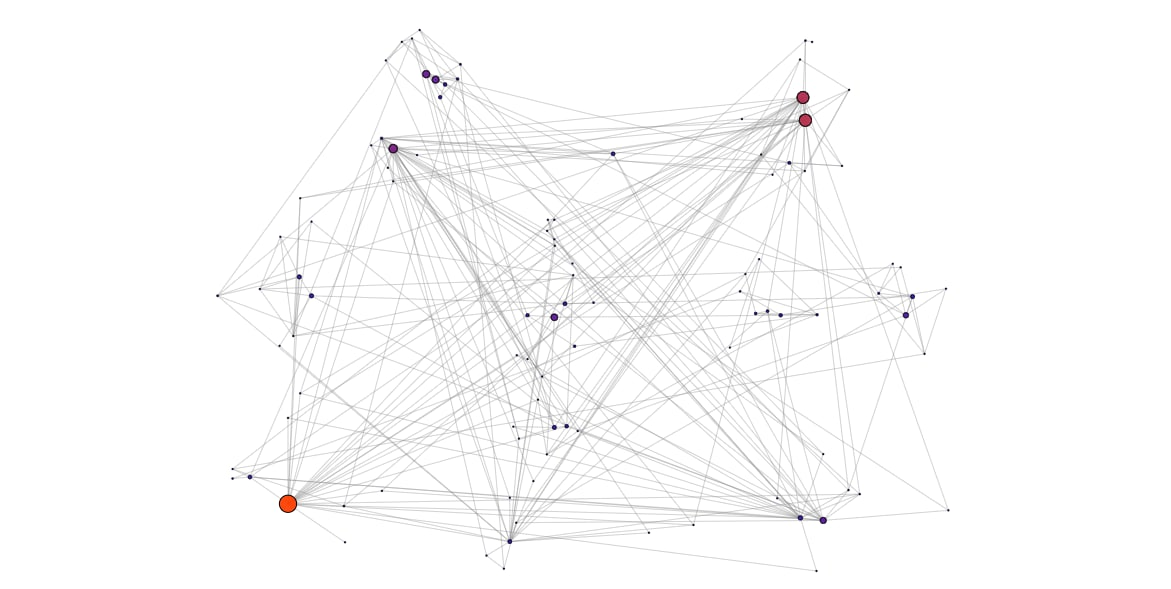
\includegraphics[width=1\textwidth]{img/graf} % width
	\caption{Полученный граф по варианту 11}
	\label{img:graf}
\end{figure}